techniques\section{Results}
First we compare and contrast the performance of our jump points
pruning algorithm with the Swamps method of
\citeauthor{pochter10}~\shortcite{pochter10}. 
Both Swamps and jump points belong to the same family of methods:
optimality preserving pruning techniques for speeding up pathfinding.
When evaluating Swamps we used the authors'
source code and ran all experiments using their recommended running parameters:
a swamp seed radius of 6 and ``no change limit'' of 2. 
\par
Next, we compare and contrast the performance of jump points pruning 
against the HPA* algorithm of \citeauthor{botea04}~\shortcite{botea04}.
Though sub-optimal, HPA* is very fast and therefore widely applied in video
games. We compare against it to establish whether or not jump points are 
equally applicable in similar contexts. 
When evaluating HPA* we used our own implementation of the algorithm which we 
configured with a fixed cluster size of 10 (as recommended by the original authors).
\par
We discuss performance in terms of search times and compare 
the average speedup experienced by A* when running with and
without pruning methods applied to the map.  
Using this metric a speedup of 2.0 is twice as fast (higher is better).

\begin{figure*}[t]
   \begin{center}
	   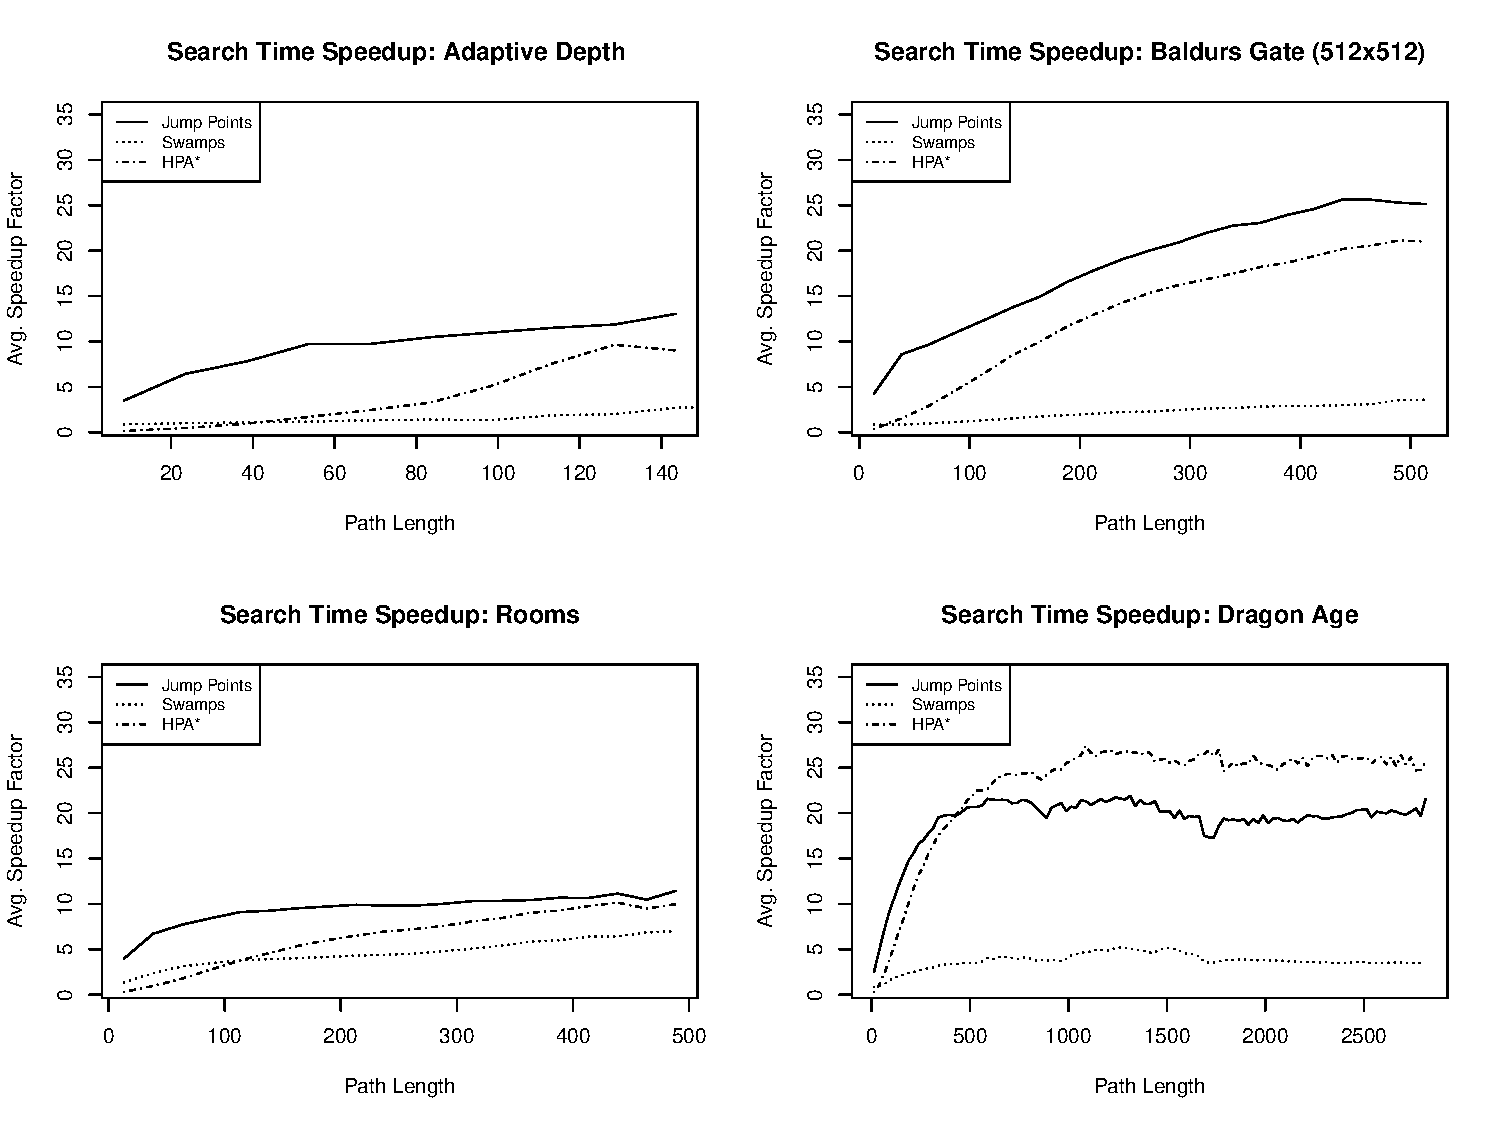
\includegraphics[width=2.0\columnwidth, trim = 10mm 10mm 10mm 0mm]
		{diagrams/speedup.pdf}
   \end{center}
   \caption{Average A* speedup on each of our four benchmarks. 
	Results are given in terms of relative search time improvement.}
\label{fig:speedup}
\end{figure*}

\textbf{Comparison with Swamps: }
As per Figure \ref{fig:speedup}(A-D), jump point pruning shows a convincing
improvement over Swamps across all benchmarks. 
The largest differences are observed on Baldur's Gate and Dragon Age where jump 
points achieve between 20-26 times search speedup compared with Swamps
only attains a 3-5 times speedup.
On the Rooms benchmark the difference is smaller: jump points pruning
speeds up search by a factor of 11 while Swamps achieves a 7 times
speedup.
The observed performance characteristics are not unexpected: Swamps prune out
areas that can be avoided without introducing a detour. However, Swamps are of
little benefit if the areas which remain are large and need to be explored 
thoroughly.
By comparison, jump points pruning rapidly explores large areas by proving
that many node expansion operations are unnecessary.
\par
Since it appears that the two algorithms have complementary strengths, a natural
extension of this work would be to combine Swamps with jump points:
first, apply Swamps decomposition to identify areas that do not have to be
explored for the instance at hand. Then, apply jump points to quickly explore the
remaining search space.
\par
\textbf{Comparison with HPA*: }
As per Figure \ref{fig:speedup}(A-D), jump points pruning is shown to be 
highly competitive with HPA*.
On Adaptive Depth, Baldur's Gate and Rooms jump points are shown to have an 
advantage, improving on HPA* search times by several factors in some cases.
On the Dragon Age benchmark however this trend is reversed; HPA* speeds up
search by up to 27 times while jump points achieve a maximum speedup of 22
times.
It is interesting to note that jump point pruning achieves the largest relative
speedup on instances with smaller path lengths
($\leq 100$). Here HPA* search times are dominated by the overhead required to
insert the start and goal into the abstract graph.
As path length increases the advantage provided by jump point pruning is eroded
and, as we see on Dragon Age, HPA* eventually becomes faster.
\par
Jump points and HPA* appear to have complementary strengths.
One direction for further work would be to use jump point pruning to speed up
HPA* insertion times. Furthermore,  jump points could be used to speed up 
HPA* path refinement once an abstract solution is found.
